\begin{figure}
\centering
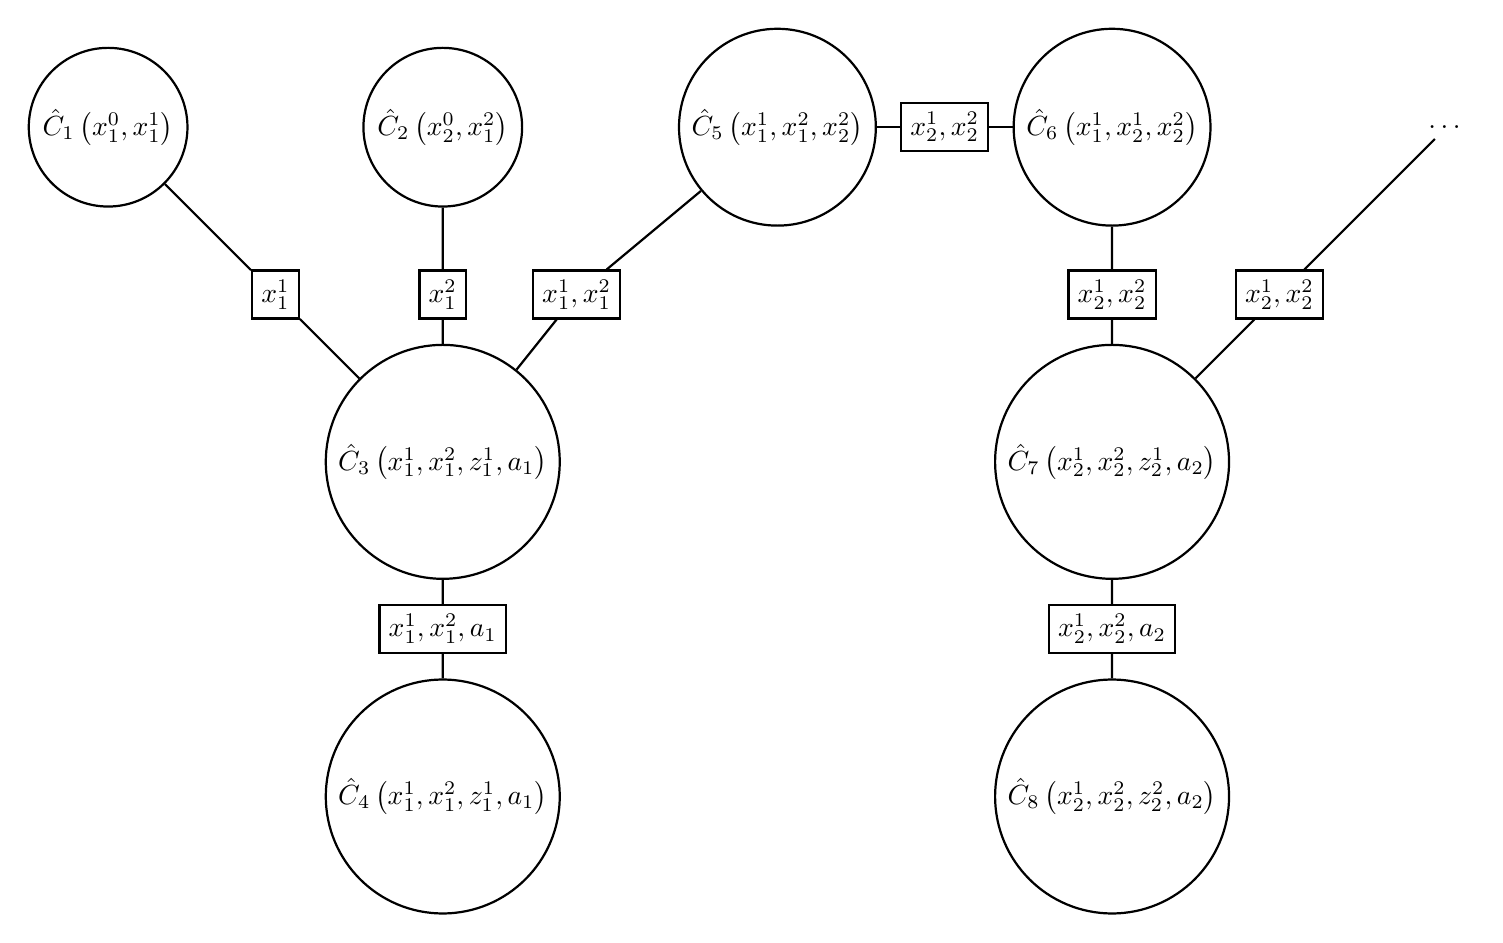
\begin{tikzpicture}[scale=0.85]
\begin{scope}[every node/.style={circle,thick,draw}]

	%Frame 1
	\node (c_1) at (0, 0) {$\pmb{\hat{C}}_{1}\left( \pmb{x}^{0}_{1}, \pmb{x}_{1}^{1} \right)$};
	\node (c_2) at (5, 0) {$\pmb{\hat{C}}_{2}\left( \pmb{x}^{0}_{2}, \pmb{x}_{1}^{2} \right)$};
	\node (c_3) at (5, -5) {$\pmb{\hat{C}}_{3}\left( \pmb{x}^{1}_{1}, \pmb{x}_{1}^{2}, \pmb{z}_{1}^{1}, a_{1} \right)$};
	\node (c_4) at (5, -10) {$\pmb{\hat{C}}_{4}\left( \pmb{x}^{1}_{1}, \pmb{x}_{1}^{2}, \pmb{z}_{1}^{1}, a_{1} \right)$};
	
	%Frame 2
	\node (c_5) at (10, 0) {$\pmb{\hat{C}}_{5} \left( \pmb{x}^{1}_{1}, \pmb{x}_{1}^{2}, \pmb{x}_{2}^{2}  \right)$};
	\node (c_6) at (15, 0) {$\pmb{\hat{C}}_{6} \left( \pmb{x}_{1}^{1}, \pmb{x}_{2}^{1}, \pmb{x}_{2}^{2}  \right)$};
	\node (c_7) at (15, -5) {$\pmb{\hat{C}}_{7} \left( \pmb{x}_{2}^{1}, \pmb{x}_{2}^{2}, \pmb{z}_{2}^{1}, a_{2} \right)$};
	\node (c_8) at (15, -10) {$\pmb{\hat{C}}_{8} \left( \pmb{x}_{2}^{1}, \pmb{x}_{2}^{2}, \pmb{z}_{2}^{2}, a_{2} \right)$};

\end{scope}

\begin{scope}[every node/.style={thick,draw}]
	%Frame 1
	\node (s_1^3) at (2.5, -2.5) {$\pmb{x}_{1}^{1}$};
	\node (s_2^3) at (5, -2.5) {$\pmb{x}_{1}^{2}$};
	\node (s_3^4) at (5, -7.5) {$\pmb{x}_{1}^{1}, \pmb{x}_{1}^{2}, a_{1}$};
	\node (s_3^5) at (7, -2.5) {$\pmb{x}_{1}^{1}, \pmb{x}_{1}^{2}$};
	
	%Frame 2
	\node (s_5^6) at (12.5, 0) {$\pmb{x}_{2}^{1}, \pmb{x}_{2}^{2}$};
	\node (s_6^7) at (15, -2.5) {$\pmb{x}_{2}^{1}, \pmb{x}_{2}^{2}$};
	\node (s_7^8) at (15, -7.5) {$\pmb{x}_{2}^{1}, \pmb{x}_{2}^{2}, a_{2}$};
	\node (s_7^9) at (17.5, -2.5) {$\pmb{x}_{2}^{1}, \pmb{x}_{2}^{2}$};

	
\end{scope}

\begin{scope}[style={thick,draw}]
   \node (xdots) at (20, 0) {\dots};
\end{scope}


\begin{scope}[style={thick,draw}]

 %\Frame 1
 \path [-] (c_1) edge node {} (s_1^3);
 \path [-] (s_1^3) edge node {} (c_3);
 
 \path [-] (c_2) edge node {} (s_2^3);
 \path [-] (s_2^3) edge node {} (c_3);
 
 \path [-] (c_3) edge node {} (s_3^4);
 \path [-] (s_3^4) edge node {} (c_4);

 \path [-] (c_3) edge node {} (s_3^5);
 \path [-] (s_3^5) edge node {} (c_5);
 
 %\Frame 2
 \path [-] (c_5) edge node {} (s_5^6);
 \path [-] (s_5^6) edge node {} (c_6);
 
 \path [-] (c_6) edge node {} (s_6^7);
 \path [-] (s_6^7) edge node {} (c_7);
 
 \path [-] (c_7) edge node {} (s_7^8);
 \path [-] (s_7^8) edge node {} (c_8);
 
 \path [-] (c_7) edge node {} (s_7^9);
 \path [-] (s_7^9) edge node {} (xdots);
	
\end{scope}

\end{tikzpicture}

\caption[The Junction Tree equivalent of Figure~\ref{figure:bayes_net}.]{The Junction tree equivalent of Figure~\ref{figure:bayes_net}, naively constructed from the cliques in Figure~\ref{figure:induced}.}
\label{figure:junction_tree}
\end{figure}